\subsection{Sequence Diagram}

This sequence diagram (see Figure~\ref{fig:sequencediagram}) illustrates the process of retrieving the details of a specific book.
The user sends a GET request to the web server with the URI \texttt{/books/5}, where \texttt{5} represents the book's ID. Upon receiving the request, the web server instantiates the \textit{BookServlet} and calls its \texttt{init(ServletConfig)} method to initialize the servlet (if it hasn't been initialized yet). After that, the server calls the \texttt{service(HttpServletRequest, HttpServletResponse)} method, which forwards the request to the \texttt{doGet(HttpServletRequest, HttpServletResponse)} method implemented in \textit{BookServlet}.
Inside the \texttt{doGet} method, the servlet obtains a database connection by invoking the \texttt{getConnection()} method inherited from \textit{AbstractDatabaseServlet}. With the active connection and the book ID, it creates a new instance of \textit{GetBookByIdDAO}.
The servlet then calls the \texttt{access()} method on the DAO. This triggers the \texttt{doAccess()} method, which prepares and executes an SQL \texttt{SELECT} query to retrieve the book with the specified ID. The result is then used to instantiate a \textit{Book} object. The DAO returns this object back to the servlet.
Once the servlet receives the book data, it sets it as a request attribute (\verb|book_details|) and forwards the request to the JSP page \texttt{bookDetails.jsp}, which is rendered and returned to the user as an HTML page.


Figure~\ref{fig:addtocartsequencediagram} shows the sequence diagram for adding a book to the shopping cart. The process starts when the user sends a \texttt{POST} request to the web server at \texttt{/cart/add/{bookId}}. The server passes the request to the \textit{CartServlet}, which runs the \textit{doPost()} method. The servlet gets the \textit{userId} from the current session. If the user is not logged in, they are redirected to the login page. Otherwise, the servlet reads the \textit{bookId} from the request.

Next, the servlet calls the \textit{getOrCreateCartId(userId)} method. It creates a \textit{GetCartByUserIdDAO} to get the user's cart from the database. In this version, we assume the cart already exists and use its \textit{cartId}. Then, the servlet creates an \textit{AddBookToCartDAO} with the connection, \textit{bookId}, and \textit{cartId}. The DAO adds the book to the cart using an SQL \texttt{INSERT} query. Finally, the user is redirected to the \texttt{/cart} page.

\clearpage
\begin{figure}[h!]
    \centering
    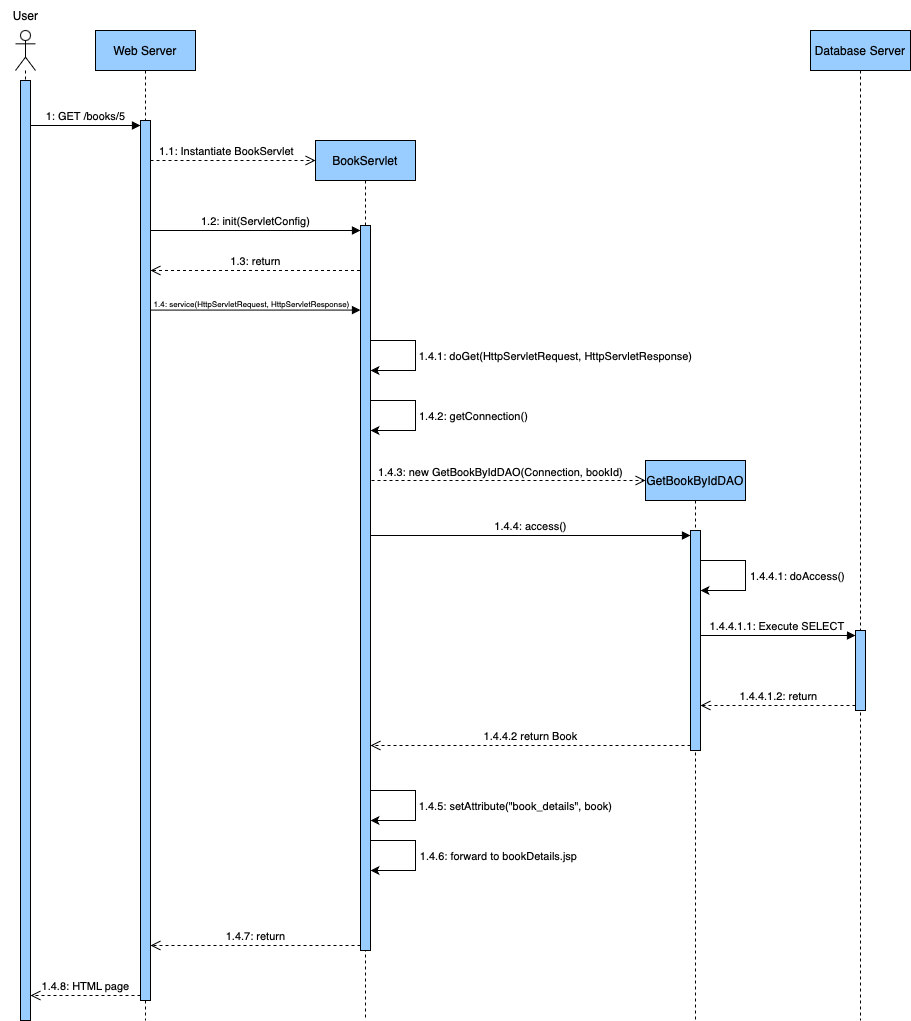
\includegraphics[width=\textwidth]{photos/SequenceDiagram.png}
    \caption{Sequence Diagram for retrieving a book by ID}
    \label{fig:sequencediagram}
\end{figure}


\clearpage
\begin{figure}[h!]
    \centering
    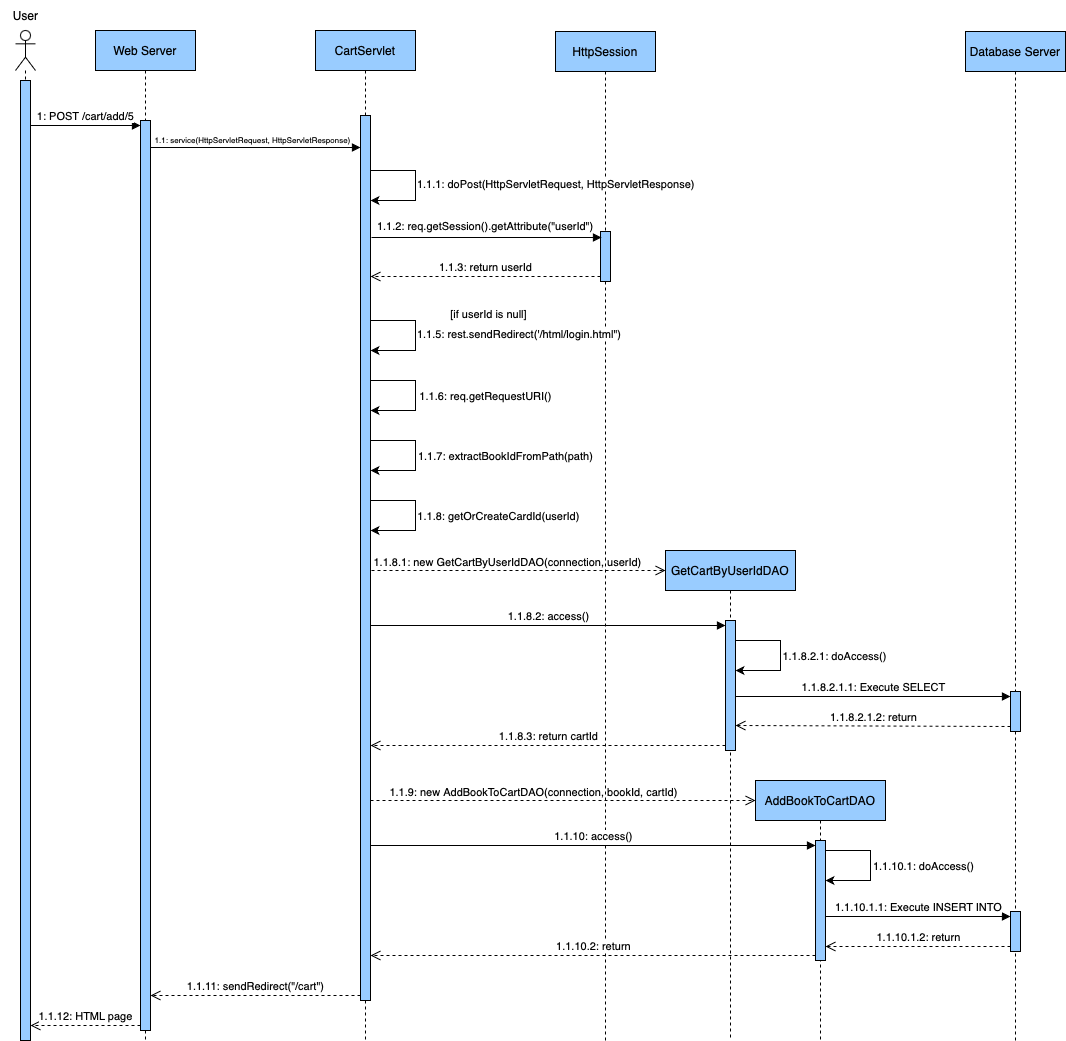
\includegraphics[width=\textwidth]{photos/SequenceDiagram_CartServlet_AddBookToCart.png}
    \caption{Sequence Diagram for adding a book to the cart}
    \label{fig:addtocartsequencediagram}
\end{figure}
